\documentclass{bioinfo}
\copyrightyear{2020} \pubyear{2020}
\usepackage{booktabs}

\access{Advance Access Publication Date: Day Month Year}
\appnotes{Manuscript Category}

\begin{document}
\firstpage{1}

\subtitle{Sequence analysis}

\title[sgRNA on-target activity prediction]{AttCRISPR : a spacetime interpretable model for prediction of sgRNA on-target activity}
\author[Xiao \textit{et~al}.]{Liming Xiao\,$^{\text{\sfb 1}}$, Yunqi Wan\,$^{\text{\sfb 1}}$ and Zhenran Jiang\,$^{\text{\sfb 1,}*}$}
\address{$^{\text{\sf 1}}$School of Computer Science \& Technology, East China Normal University, Shanghai, 200062, China.}

\corresp{$^\ast$To whom correspondence should be addressed.}

\history{Received on XXXXX; revised on XXXXX; accepted on XXXXX}

\editor{Associate Editor: XXXXXXX}

\abstract{\textbf{Motivation:} More and more Cas9 variants with higher specificities are developed to avoid the off-target effect, which bring a significant volume of experimental data. 
Conventional machine learning performs poorly on these datasets, while the methods based on deep learning are often lack of interpretability, 
which makes researchers have to trade-off accuracy and interpretability. 
It is necessary to develop a method which can not only match deep learning based methods in performance, 
but also with strong interpretability that can be comparable to conventional machine learning methods.\\
\textbf{Results:} To overcome these problems, we design and implement AttCRISPR, an intrinsic interpretable method based on deep learning to predict the on-target activity. 
The advantage of AttCRISPR lies in using the ensemble learning strategy to stack available encoded-based methods and embedded-based methods with strong interpretability. 
Comparison with the state-of-the-art methods (WT-SpCas9, eSpCas9(1.1), SpCas9-HF1), AttCRISPR can achieve an average spearman value of 0.872, 0.867, 0.867, respectively on several public datasets, which is superior to these methods. 
Furthermore, benefits from two attention modules, spatial and temporal attention modules, AttCRISPR has strong interpretability. 
Through them, we can understand the decisions made by AttCRISPR at both global and local levels without other post hoc explanations techniques. 
With the trained model, we reveal the preference for each position-dependent nucleotide on the sgRNA (small guide RNA) sequence in each dataset at global level. 
And at local level, we prove that interpretability of AttCRISPR can be used to guide researcher to design sgRNA with higher activity. \\
\textbf{Availability:} The example code are available at \href{https://github.com/South-Walker/AttCRISPR}{https://github.com/South-Walker/AttCRISPR}\\
\textbf{Contact:} \href{zrjiang@cs.ecnu.edu.cn}{zrjiang@cs.ecnu.edu.cn}\\
\textbf{Supplementary information:} Supplementary data are available at \textit{Bioinformatics}
online.}

\maketitle

\section{Introduction}

Clustered regularly interspaced short palindromic repeats (CRISPR) / CRIPSR associated protein 9 (Cas9) systems are preferred over other biological research and human medicine technologies now, 
beacuse of it's efficiency, robustness and programmability. 
Cas9 nucleases can be directed by short guide RNAs (sgRNAs) to introduce site-specific DNA double-stranded breaks in target, 
so to enable editing site-specific regions within genome \citep{jinek2012a,cong2013multiplex,mali2013rnaguided}. 
CRISPR/Cas9, to a large extent, has developed genetic therapies at the cellular level, 
while there are still severe medical disadvantages even now which has greatly hindered the further clinical application of the CRISPR/Cas9 systems. 
One of these disadvantages is due to unexpected insertion and deletion caused by off-target effect \citep{rubeis2018risks,kang2016introducing,ishii2017reproductive,liang2015crispr/cas9-mediated}. 
To overcome this disadvantage, a solution is to engineer CRISPR / Cas9 with higher specificities. 
That's why more and more higher specificities Cas9 variants, such as enhanced SpCas9 (eSpCas9(1.1)), 
Cas9-High Fidelity (SpCas9-HF1) \citep{slaymaker2016rationally,ishii2017reproductive}, hyper-accurate Cas9 (HypaCas9) \citep{kleinstiver2016high-fidelity}, 
been developed and bring a significant volume of experimental data, which means that researchers have to face the difficulty of analyzing such huge and heterogeneous data.

The activity of chosen sgRNA sequence determines the efficiency of genome editing, 
however distinctly fluctuant behaviors have been observed for the performance of different sgRNAs, even in the same Cas9 system. 
This fact indicates that it's meaningful to explore an efficient approach to predict sgRNA activity and even guide sgRNA design. 

In practice, there have been a number of applications and toolkits applied in this task. In the earlier studies, the methods \emph{in silico} are categorized into three types: 
(1) alignment-based, (2) hypothesis-driven and (3) learning-based \citep{chuai2018deepcrispr}. 
Recently, we noticed that the last type of method seems to be getting more attention because of huger and huger datasets \citep{liu2019computational}. 

Learning-based method, which designed to predict the on-target activity (or off-target probability) of sgRNAs, 
is essentially a computational model built by machine learning algorithms, not only conventional machine learning but also deep learning. 
In general, the single or multiple base sequences (vary according to the task) and biological features are represented as a multi-dimensional vector $X\in\mathbb{R}^d$, 
and $d=l+b$, where $l$ refers to the length of base sequences and $b$ refers to the number of biological features, these methods can be represented as
\begin{equation}
 y=Score( X)\label{eq:01}
\end{equation}
 where $Score(\cdot)$ depends on the algorithm being selected, and $y$ denotes the predicted value.
 Some studies on HT\_ABE and HT\_CBE (two gene editing tools grew out of CRISPR) have shown that deep learning based models often outperformed conventional machine learning, when the number of sgRNAs in the dataset reached a certain level \citep{kim2018deep,kim2019spcas9,Song2020}. 
 Per contra, conventional machine learning algorithms, such as linear regression, logistic regression and the decision tree, are often more interpretable due to the fewer parameters and clearer mathematical assumptions. 
 In short, what was needed for developer is to trade-off accuracy and interpretability. 
 \citeauthor{MuhammadRafid2020} consider deep-learning models as black boxs and believe they lack interpretability, 
 motivated by the empirical assertion, they turn to build a model based on conventional machine learning to compete with state-of-the-art deep learning models \citep{MuhammadRafid2020}. 
 On the other hand, input perturbation based feature importance analysis become a preferred components to reveal the importance of features in deep learning models. 
 \citeauthor{Liu2019} use a sliding window of length 2 to extract dimeric as input and rank the position of dimeric by contribution to final output \citep{Liu2019}. 
 One regret is that subject to the processing of the input sgRNA sequence, their analysis can not exactly on the nucleotide class. 
 Further, SHAP, one of the most prominent of model explain techniques, has been widely used to understand the decision made by the model. 
 \citeauthor{wang2019optimized} develope DeepHF, a deep learning based model, and use Deep SHAP to revealed nucleotide contributions \citep{wang2019optimized}. 
 Deep SHAP is a compositional approximation of SHAP values since it is challenged to computate SHAP values exactly, especially for a complex deep neural networks. 
 In our understanding, the method based on input perturbation often requires better generalization ability of the model (even for artificial ridiculous noise data). 

 In addition, the interpretability of existing models are all at global level, and result is a general pattern in the datasets. 
For example, which position has a great impact on the final decision of the model and which position-dependent nucleotide has a positive impact on the activity. 
Lack of analysis at local level. 
For example, which structure causes the low activity of a certain nucleotide sequence and how to improve its activity with a few modification. 
In light of the above, we believe it is critical to develop an effective model which can not only have good performance, but also with strong interpretability.


\begin{figure}[!tpb]%figure2
    \centerline{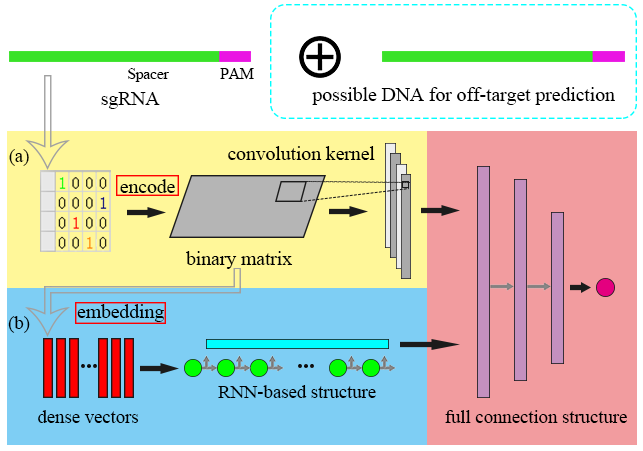
\includegraphics[width=86mm]{NEWcategory.png}}
    \caption{Two categories of the deep learning models used in sgRNA related task. 
    (a) Model work in spatial domain. 
    In spatial domain, the base sequence is encoded into a binary matrix (or a binary image). 
    Since convolution has great advantages in extracting spatial features, the CNN is an excellent tool in spatial domain. 
    (b) Model work in temporal domain. 
    In temporal domain, the base sequence (represented by the binary matrix) is embedded into a sequance of high-dimensional vector, 
    in which the RNN perform better.
    In addition, we note that the last layers of neural network are usually full connection structure (not necessarily), 
    which greatly increases the difficulty of understanding the decisions of model.
    }\label{fig:category}
\end{figure}

Deep neural network has shown its power in the study of CRISPR/Cas9 and its improved systems \citep{liu2019computational}. 
Most of the deep neural networks existing are the combination of recurrent neural network (RNN), convolutional neural network (CNN), fully connected neural network (FNN), and their variants. 
As Figure~\ref{fig:category} show,  
we found that the deep learning models used in sgRNA on-target activity (even for off-target effect) prediction tasks in recent years can be divided into the following two categories according to the encoding approach of the sgRNA sequence (sgRNA-DNA sequence pair, for off-target effect prediction):

\begin{enumerate}
    \item Methods in spatial domain. 
    Some previous studies have used the methods based CNN to predict sgRNA on-target activity or off-target effect \citep{chuai2018deepcrispr,kim2018deep,lin2018off-target}. 
    They process sgRNA base sequence inputs with the help of one-hot encoding idea. 
    In other words, they regard it as two-dimensional image data, and use convolution layer to extracte potential features in spatial domain, 
    It is worth noting that \citeauthor{zhang2020c-rnncrispr:} adds bidirectional gated recurrent unit (BGRU, in short), a RNN variant, after pooling layer of classic CNN network \citep{zhang2020c-rnncrispr:}. 
    Our explanation is that BGRU assists CNN to extract spatial features in one dimension, under this belief it belong to this category. 
    \item Methods in temporal domain. 
    Although RNN-based network have been shown effective to improve the performance of the model with temporal sequential input, especially in Natural Language Processing(NLP) and sequential recommendation, 
    RNN be not used for gRNA activity prediction, until recently \citep{Liu2019,wang2019optimized,liu2020deep}. 
    They consider the nucleotides(can also dimer or polymer) in the sgRNA sequence as word, and the sgRNA sequence itself as a sentence (from 5' to 3'), then a trainable matrix (could be either supervised or unsupervised) is used to project the word to the dense real-valued space. 
    This technology is called embedding, which generates the base embedding. RNN further encoding the base embedding into a sequence of hidden state vector. 
    Specially, \citeauthor{Liu2019} use RNN and CNN in parallel to extract features in base embedding \citep{Liu2019}. 
    However, base embedding is not spatially interpretable (different from one-hot encode), and they have no way to further explore the correlation between CNN and RNN output. 
    Almost all of the RNN based models used in sgRNA on-target activity or off-target effect flatten the hidden state vector into a one-dimensional vector as the input of the fully connected layer. 
    It is a pity that the temporal sequential dependency of hidden state vector are rarely noticed. 
    In summarize, RNN has limited representation power in capturing spatial feature. 
    Furthermore, the hidden state vector representation is usually hard to understand.
\end{enumerate}

Attention mechanism has demonstrated its power in NLP, Statistical Learning, Speech and Computer Vision. 
 It makes model tends to focus selectively on parts of the input, which is help in performing the task effectively. 
 Previous observation have shown that Cas9 preferentially binds sgRNAs containing purines but not pyrimidines \citep{wang2014genetic} and multiple thymine in the spacer impairing sgRNA activity \citep{wu2014genome-wide}, 
 that is to say some specific nucleotides and base position need more attention compared to others. 
 The above is the premise of introducing attention mechanism. Strictly speaking, we are not the first to bring attention mechanisms into this field. 
 The most similar approach to ours is the work based on transformer by \citeauthor{Liu2019}. 
 They use transformer, a components based on attention mechanism, instead of RNN to improve the ability of temporal feature extraction, 
 hence, enhance the performance of their model \citep{vaswani2017attention,Liu2019}. 
 In our work,the interpretability benefit from attention mechanism is more focused. 
 Our main contributions are as follows:\vspace*{1pt}
\begin{itemize}
    \item Present a novel deep-learning model, which can extract potential feature representation of sgRNA sequence in both spatial and temporal domain parallelly. 
    Finally, the ensemble learning method is used to combine the two to achieve better performance than current state-of-the-art models. 
    \item Introduce attention mechanism into our model. 
    As a result, it does not need post hoc explanations techniques based on input perturbation to explain itself. 
    It is intrinsic interpretable in both temporal and spatial domains.
    In the spatial domain it's at global level, while at local level in the temporal domain. 
    Thus, it is transformed from a black box to an intrinsically interpretable model with the performance of deep learning based model. 
    \item Throught ablation analysis and testing a series of possible network structures, 
    we find there are multiple components and strategies can improve the performance of AttCRISPR, 
    which could outperform current state-of-the-art tools on DeepHF dataset.\vspace*{1pt}
\end{itemize}

\section{Materials and methods}
\subsection{Datasets}

The dataset we used for training, validation and testing is built by \citeauthor{wang2019optimized}. 
We extracted 55604, 58617, 56888 sgRNAs with activity (represented by insertion/deletion (indel)) for WT-SpCas9, eSpCas9(1.1) and SpCas9-HF1, respectively, from its source data. 

\subsection{Sequence encoding and embedding}

For encoding process, we use the complementary base to represent the original base in sgRNA. 
Further, we use one-hot encode strategy, that is to say, we encoding each base in sgRNA into a four-dimensional vector 
(encode A,T,G,C into [1,0,0,0], [0,1,0,0], [0,0,1,0], [0,0,0,1], respectively), called one-hot vector. 
Then a sgRNA can be considered as a matrix $X_{oh}\in\mathbb{R}^{l\times4} $, named one-hot matrix (a little sparse, since an one-hot vector is zero in all but one dimension). 
We believe it is meaningful to regard $X_{oh}$ as a binary image, 
therefore, it is used as an input of CNN, which performs well in the image field.
Meanwhile, as mentioned above, one-hot matrix is a little sparse. 

To facilitate the training process, we can mapping each one-hot vector into a dense real-valued high-dimensional space, which is called embedding. 
In summarized, at the matrix level, the formula is as follows
\begin{equation}
X_e=X_{oh}E_m\label{eq:08}
\end{equation}
where $X_e$ named embedding matrix, $E_m\in\mathbb{R}^{4\times m}$ is a trainable transformational matrix, $m$ refers to the dimension of embedding space. 
We believe it is also meaningful to regard nucleotides in the sgRNA sequence as word, and the sgRNA sequence itself as a sentence, 
Guided by this belief $E_m$ is the word embedding matrix and $X_e$ is the sentence embedding in NLP.
Therefore, $X_e$ is used as an input of RNN (or its variant), which performs well in the NLP field.

Due to each element of $X_{oh}$ is interpretable (representing whether there is a corresponding nucleotide type at the corresponding location), 
we call $X_{oh}$ the spatial input, and the CNN work on $X_{oh}$ is the method in spatial domain. 
In other hand, different from $X_{oh}$, $X_e$ can only be explained in the first dimension (representing the embedding vector of corresponding nucleotide type), 
and embedding vector is difficult for humans to understand. 
That's why we call $X_e$ the temporal input, and the RNN (or its variant) work on $X_e$ belongs to the method in temporal domain. 

\subsection{Neural network architecture}

Based on the categorization above, we assume that the method in spatial domain and in temporal domain are heterogeneous, 
which can satisfy the diversity premise of ensemble learning. 
Based on the assumption above and ensemble learning, we follow the stacking strategy to develop AttCRISPR 
which can extract potential feature representation of sgRNA sequence in both spatial and temporal domain parallelly. 
Further, we apply attention mechanisms in both spatial and temporal domain to enhance the interpretability of AttCRISPR.

\subsubsection{First-order preference and second-order preference}

In order to introduce the neural network architecture of AttCRISPR, Let's define first-order preference and second-order preference for convenience. 
Taking a simple linear regression model as an example, for input $X$ in Equation~(\ref{eq:01}), $y$ in Equation~(\ref{eq:01}) is as following
 \begin{equation}
y = AX\label{eq:linear}
\end{equation}
where $A \in\mathbb{R}^d$, the total differential of $y$ in Equation~(\ref{eq:linear}) is as following
 \begin{equation}
dy = \sum^{d}_iA_idX_i\label{eq:02}
\end{equation}
where $A_i$ and $X_i$ denotes the $i$-th dimension of the vector $X$ and $A$, 
$A_i$ indicates how dramatically the function changes as $X_i$ changes in a neighborhood of $X$, 
in other words, the importance of $X_i$. 
That's why we'll call $A$ first-order preference in our paper. 
Specifically, we use a vector $A_i$ to build the first-order original preference at position $i$ within sgRNA sequence, 
and $X_i$ is an embeddedness of the $i$-th feature, then $A$ and $X$ are two matrix. 
Further, the final result can be weighted by a trainable non-negative weight vector $W\in\mathbb{R}^l$, as follow
\begin{equation}
y=W \cdot AX^{T}\label{eq:superlinear}
\end{equation}
then we define $\tilde{A}$ as the first-order combine preference matrix (or just first-order preference), which means $\tilde{A}$ can be expressed linearly by $A$ as follow
\begin{equation}
\tilde{A}=BA\label{eq:04}
\end{equation}
where the weight matrix $B\in\mathbb{R}^{l\times l}$ is learned through attention mechanism, 
which we'll call the second-order preference matrix in our paper due to its calculation is based on first-order preference, 
it can explain how a particular pattern containing two nucleotides affects the base sequence. 
Then the predicted value can be expressed as
\begin{equation}
y=W \cdot \tilde{A} {X_e}^{T}\label{eq:05}
\end{equation}

\subsubsection{Method in spatial domain}

\begin{figure}[!tpb]%figure2
    \centerline{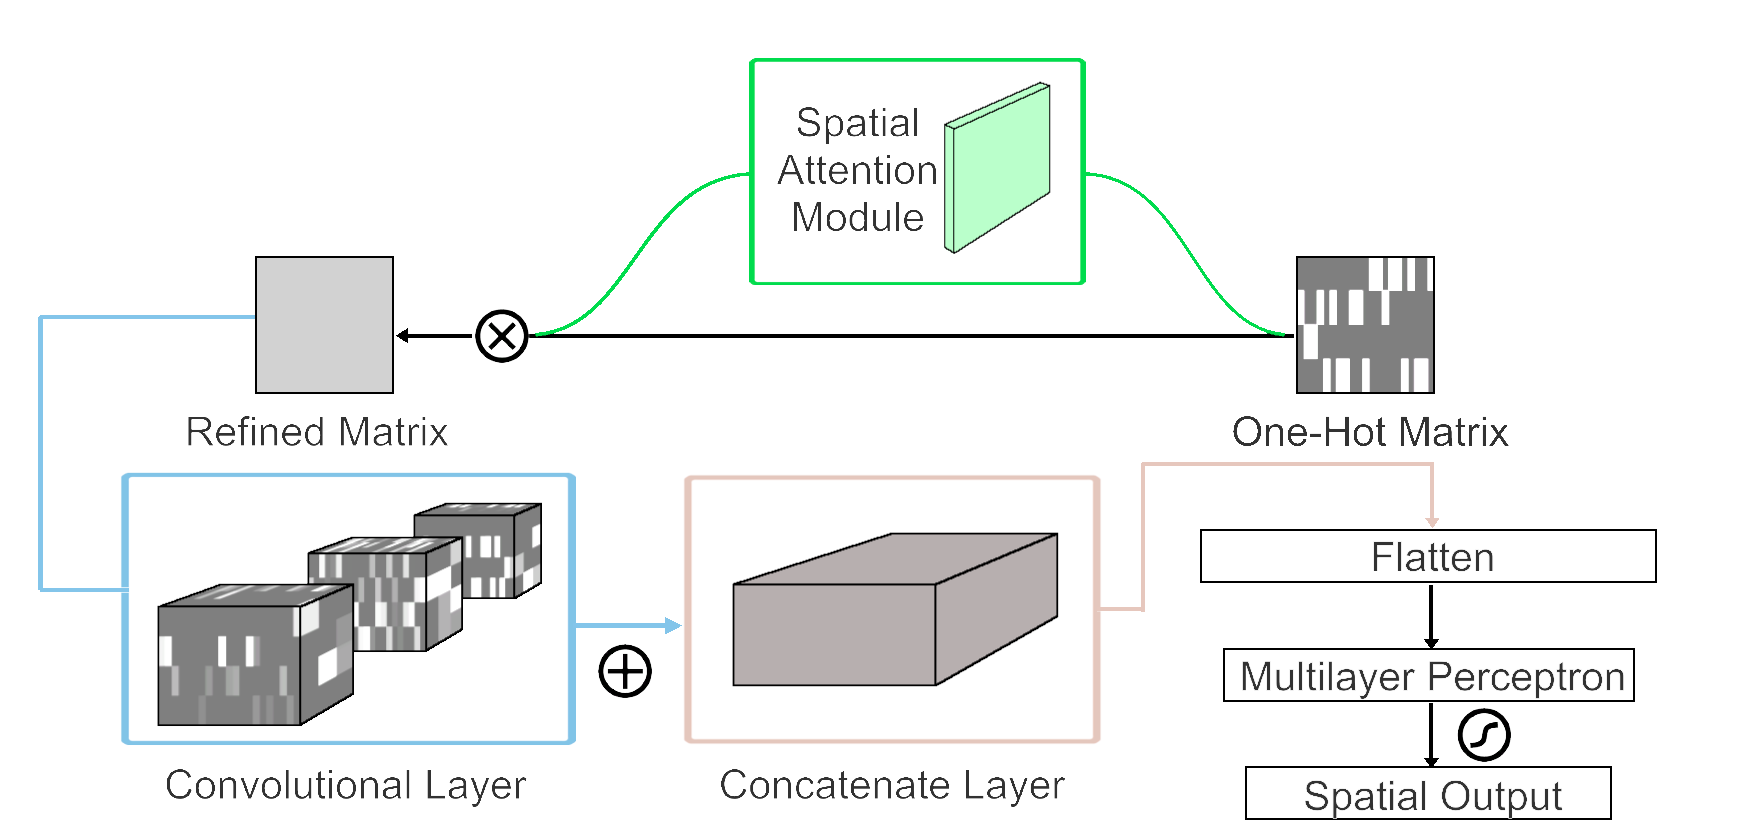
\includegraphics[width=86mm]{CNNv2.png}}
    \caption{The architecture of spatial domain method in AttCRISPR. 
    The input of the method is encoded sgRNA sequence $X_{oh}$, a $21\times 4$ one-hot matrix. 
    Then refine it through a spatial attention module, which could tell us the importance of a specific matrix element (or just say, pixel).
    A simple CNN followed is applied to extract potential feature representation of sgRNA sequence.
    In the last step, we flatten the output of CNN network into a one dimensional vector and 
    use a multilayer perceptron with sigmoid activation function to achieve the spatial output $y_s$.}\label{fig:CNN}
\end{figure}
As Figure~\ref{fig:CNN} demonstrated, the method in spatial domain relies on the CNN. 
As previously mentioned, sgRNA sequence has been encoded into a $21\times 4$ one-hot matrix $X_{oh}$, and we regard $X_{oh}$ as a binary image. 
Then, convolution kernels with different size are used to extract potential spatial features just like what other do in computer vision. 
According to the foregoing, the spatial attention module proposed by \citeauthor{woo2018cbam:} can be applied in our method, 
which has been used to improve the performance of CNN in vision tasks.

\begin{figure}[!tpb]%figure3
    \centerline{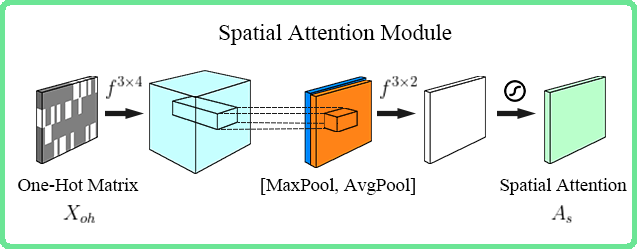
\includegraphics[width=86mm]{spatialmodule.png}}
    \caption{Details of spatial attention module. A convolution layer is used to generate multi-channel map from $X_{oh}$.
    Then concatenated the output of both max-pooling and average-pooling method and forward it to the last convolution layer.
    A sigmoid function is used to map the final result to a range of zero to one at last, 
    which generates the spatial first-order preference matrix $A_s$.
    }\label{fig:spatialmodule}
\end{figure}

As shown in Figure~\ref{fig:spatialmodule}, given an one-hot map $X_{oh}$, spatial attention module generating spatial attention matrix 
$A_s\in\mathbb{R}^{l\times 4}$ with the same as $X_{oh}$ in shape. 
Each element of $A_s$ is constrained to a range of zero to one, implemented by a sigmoid function, which reflects the importance of the corresponding elements of $X_{oh}$.
The overall spatial attention process can be summarized as:
\begin{equation}
\left\{\begin{array}{l}
X_{mc} = f^{3\times4}(X_{oh})
\\A_s = \sigma(f^{3\times2}([AvgPool(X_{mc});MaxPool(X_{mc})]))
\\X_{rf} = A_s\otimes X_{oh}
\end{array}\right.\label{eq:11}
\end{equation}
where $f^{p\times q}$ represents a convolution operation with the filter size of $p\times q$, 
$p,q\in\mathbb{Z}^{+}$, $X_{mc}$ is a multi-channel map generated by $X_{oh}$, $\sigma$ denotes the sigmoid function, 
AvgPool denotes the average-pooling operation, MaxPool denotes the max-pooling operation, $\otimes$ denotes element-wise multiplication.
Spatial attention matrix $A_s$ formally conforms to our proposed definition of first-order preference (each element of $X_{oh}$ is multiplied by the corresponding element of $A_s$), 
in other words, element of $A_s$ reveal how important the corresponding elements in $X_{oh}$ is. 
We think it can reveal the preference of the scoring function at each position. 
For instance, follow the encoding rules above, we train spatial domain part of AttCRISPR with the WT-SpCas9 dataset. 
Then take the average of all spatial attention matrix, and the element in the first row and third column are closer to 1, which means when calculate the final score, 
G typically may have a important contribution at first position within sgRNA sequence. 
In fact, this corresponds to some early studies concerning the Human (hU6) promoter, which is believed to require G as the first nucleotide of its transcript \citep{jinek2012a,cong2013multiplex,mali2013rnaguided}.

\subsubsection{Method in temporal domain}
As Figure~\ref{fig:04} show, temporal domain part of AttCRISPR relies on the RNN (or its variant). 
As previously mentioned, we mapping each one-hot vector into a dense real-valued high-dimensional space follow the Equation~(\ref{eq:08}), which generates the embedded matrix $X_e$.
And we regard $X_{e}$ as a sequential data, or temporal data.
RNN (or its variant) has showed outstanding performance in the tasks with temporal data (for instance, NLP, sequential recommendation). 
That's why we prefer to use it to extract potential temporal features. 
To be precise, we prefer the architecture of encoder-decoder which has been proven to be effective in Seq2Seq task. 
Two main differences we have to face are that sgRNA is not a natural language in the traditional sense, and we don't have to translate it to other sequence. 
To accommodate them, the embedded matrix $X_e$ is used as input of both the encoder and decoder, and the sequence of decoder is to build the first-order preference of sgRNA sequence $\tilde{A}$. 
As mentioned above, the predicted value $y$ should satisfy Equation~(\ref{eq:05}). 

On this basis, we apply the idea of attention mechanism which has been widely used in NLP tasks to AttCRISPR in the method of temporal domain, 
and name it temporal attention module \citep{luong2015effective,vaswani2017attention}.
According to the idea of \citeauthor{vaswani2017attention}, temporal attention module satisfies the following equation
\begin{equation}
Attention(Q,K,V)=align(Q,K)V\label{eq:13}
\end{equation}
where the $align(\cdot)$ is put forward by \citeauthor{luong2015effective}. 
$Q$, $K$, $V$ are queries, keys and values matrix accordingly in the paper of \citeauthor{vaswani2017attention}. 

As Figure~\ref{fig:05} show, in our attention module they are calculated by the following equation
\begin{equation}
\left\{\begin{array}{l}
K_i=Encoder({X_e}_i,\theta_E,K_{i-1})
\\ Q_i=Decoder({X_e}_i,\theta_D,Q_{i-1})
\\V=K 
\end{array}\right.\label{eq:14}
\end{equation}
where vector $K_i$, $Q_i$ denotes the $i$-th row of the matrix $K$ and $Q$ accordingly, $Encoder(\cdot)$ and $Decoder(\cdot)$ are independent GRU units, $\theta_E$ and $\theta_D$ denote all the related parameters of GRU networks accordingly. 
In the actual implementation, we apply the bidirectional GRU networks for better performance, and for the sake of conciseness, we show a conventional GRU network here. 
The function $align(\cdot)$ is as follows
\begin{equation}
B=align(Q,K)\label{eq:16}
\end{equation}
\begin{equation}
B_i=softmax(Q_iK^T)\otimes G_i\label{eq:17}
\end{equation}
\begin{equation}
G_{ij}=\left\{\begin{matrix}
exp(\frac{(i-j)^2}{-2\sigma})&,\left | i-j \right |\leqslant \sigma
\\ 0&,\left | i-j \right |>  \sigma
\end{matrix}\right.\label{eq:18}
\end{equation}
where the matrix $B\in\mathbb{R}^{l\times l}$ is the second-order preference we need, and vector $B_i$ denotes the $i$-th row of the matrix $B$. 
$G\in\mathbb{R}^{l\times l}$ is the damping matrix base on Gaussian function. 
Since a simple belief that the closer the base is to the $i$-th position, the more it affects the $i$-th position normally, we use the damping matrix G to constrain the network learning. 
$\sigma$ represents a threshold of length, any base over this length from the position $i$ is not considered to be affected.
Further, if we think of the values matrix as a vector form of the first-order preference $A$ in Equation~(\ref{eq:04}), we can reach the following equation
\begin{equation}
\tilde{A}=BV\label{eq:19}
\end{equation}
according to above, values matrix $V$ comes from the hidden states of a bidirectional GRU networks, which is usually hard to understand.
While $B$ is the second-order preference matrix obtained by the attention mechanism. 
We believe that the $j$-th dimension of $B_i$, denoted as $B_{ij}$, can reveal the effect of the base at position $j$ on position $i$ in the biological sense. 
\begin{figure}[!tpb]%figure4
    \centerline{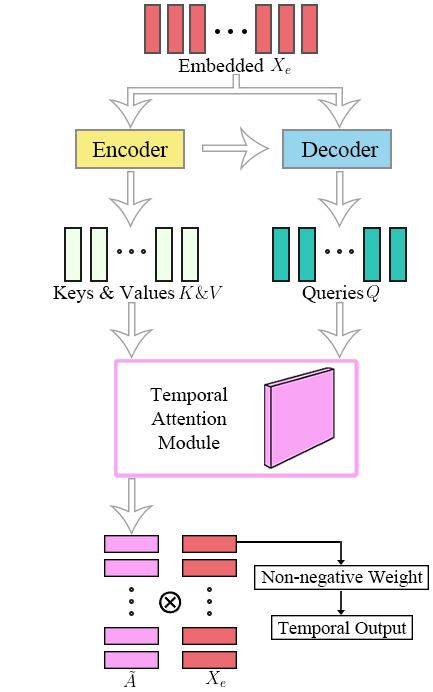
\includegraphics[width=86mm]{temporalmodule.png}}
    \caption{The architecture of temporal domain method in AttCRISPR. 
    The input of the method is embedding sgRNA sequence $X_e$, a $21\times e$ embedding matrix, where $e$ is the dimension of a nucleotide embedding vector. 
    Then Keys $K$, Values $V$ and Queries $Q$ is generated through a classic encoder-decoder structure which is need for temporal attention module.
    Next, the temporal attention module generates the first-order preference $\tilde{A}$, a $21\times e$ matrix (or a vector set). 
    Each of the row vectors in matrix $\tilde{A}$ represents the base preference of sgRNA at the corresponding position, we use their dot product with the corresponding row vector in embedded $X_e$ to build the score of corresponding position. 
    Hence, a full connection layer is used to weighted average them and achieve the temporal output $y_t$.
    }\label{fig:04}
\end{figure}
\begin{figure}[!tpb]
\centerline{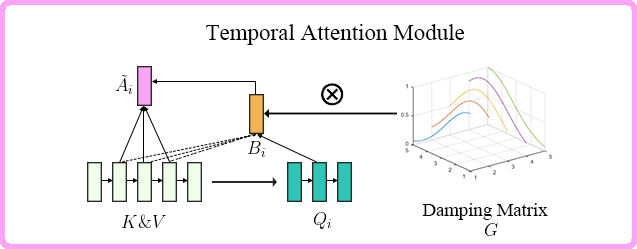
\includegraphics[width=86mm]{temporalattentionmodule.png}}
\caption{        
    Details of temporal attention module. 
    To generate the first order preference vector in the $i$ position of sgRNA $\tilde{A}_i$. 
    First, the $i$-th row vector of the querys matrix $Q_i$ is multiplied by the transpose of the keys mateix $K^T$, and apply a softmax function to obtain a preliminary weights vector on the values. 
    Second, to favor the alignment points near $i$, the weights vector obtained is multiplied element-by-element by the $i$-th row vector of the damping matrix $G$, as Equation~(\ref{eq:17}) has shown. 
    $G_{ij}$ can be regarded as the result of place a Gaussian distribution centered around $i$, then sampling the position $j$ (a scaling factor is used to ensure the sum of $G_I$ is $l$). 
    Then we achieve the second-order preference matrix $B$, it is also a weights matrix on the values. So the first-order preference matrix $\tilde{A}$ come from the product of $B$ and values matrix $V$.
    Temporal attention module generates the temporal first-order preference matrix $\tilde{A}$ and the temporal second-order preference matrix $B$.
    }\label{fig:05}
\end{figure}

\subsubsection{Ensemble model following stacking strategy}

Some indirect sgRNA features, which can't be obtained directly by deep learning, 
including position accessibilities of secondary structure, stem–loop of secondary structure, melting temperature, 
and GC content are strongly associated with sgRNA activity \citep{Wang2016ProteinSS,wang2019optimized}. 
It's worth noting that in the work of \citeauthor{wang2019optimized}, hand-crafted biological features didn't be normalized. 
Since the wide range of data distribution, we normalize it based on the standard score (Z-Score).

Then we use a simple full connection network to extract the indirect features, and call the output of fully connection network $y_{bio}$. 
As mentioned above, we assume that the method in spatial domain and in temporal domain can satisfy the diversity premise of ensemble learning.
That's why we follow the stacking strategy, to integrate the methods in time domain and space domain. 
Specifically, the $y_{bio}$, the spatial output $y_{s}$ and the temporal output $y_{t}$ we got earlier are concatenated and then weighted averaging is performed through a full connection layer as follow
\begin{equation}
y=W[y_{bio};y_s;y_t]\label{eq:20}
\end{equation}
where, $y$ is the final prediction value of AttCRISPR, $W$ is the weight learned by the full connection network. 
In the actual implementation, we freeze the network in the spatial domain and temporal domain firstly, in order to make our network focused on learning the weight $W$.
Then the parameters of the entire network are adjusted in the fine tuning of AttCRISPR.

\subsection{Current prediction methods}

As far as we know, DeepHF, the state-of-the-art method, 
achieved Spearman correlation coefficients of 0.867, 0.862 and 0.860 for WT-SpCas9, eSpCas9(1.1) and SpCas9-HF1, respectively \citep{wang2019optimized}. 
Another tool worth noting is CRISPRpred(SEQ), which is based on conventional machine learning and need complicated human feature engineering exercise \citep{MuhammadRafid2020}. 
They also test their tool with this dataset and achieved Spearman correlation coefficients of 0.838, 0.830 and 0.821 for WT-SpCas9, eSpCas9(1.1) and SpCas9-HF1, respectively (without any hyperparameter tuning).

In order to make the comparison apples to apples, we follow the same strategy as \citeauthor{wang2019optimized} to design our experiments.
To be more specific, each set is shuffled and divided into three parts, 76.5\%, 15\% and 8.5\% of the relevant data was used as the training, test and validation set respectively in a single experiment. 
The experiment is repeated ten times with the results recorded and averaged finally.

\subsection{Experiment design}

Two different experiments are carried out in our work. 
The first one is designed for ablation analysis of AttCRISPR. 
We compare the performance of end2end method (without any hand-crafted biological features) in both spatial and temporal domain. 
Furthermore, we test the ensemble method based on the same strategy to prove that the ensemble method in both spatial and temporal domain can significantly improve the performance. 

The second experiment is designed to compare the performance of AttCRISPR with other current prediction methods. 
In order to make the comparison apples to apples, we reduce the dimensionality of the same hand-crafted biological features as DeepHF's, 
which has been shown to enhance the predictability of a deep-learning model greatly, with a multilayer perceptron. 
Then follow the Equation~(\ref{eq:20}) to achieve the final prediction value. 
AttCRISPR (with the hand-crafted biological features) performs better on all three datasets than DeepHF. 

\begin{table}[!tpb]
    \processtable{The methods compared in our work and brief description of these methods\label{Tab:baseline}} 
    {\begin{tabular}{@{}lllp{3.5cm}l@{}}\toprule
        Method & Neural & End2end & Description\\\midrule
        CNN$^*$ & Yes & Yes & Naive CNN\\
        RNN$^*$ & Yes & Yes & Bidirectional long short-term memory neural network\\
        XGBoost$^*$ & No & Yes & Extreme Gradient Boosting regression tree\\
        MLP$^*$ & Yes & Yes & Multilayer perceptron\\
        DeepHF$^*$ & Yes & No & Bidirectional long short-term memory neural network (with hand-crafted biological features)\\
        CRISPRpred(SEQ)$^{\#}$ & No & No & A conventional machine learning pipeline\\
        SpAC & Yes & Yes & Spatial AttCRISPR\\
        TAC & Yes & Yes & Temporal AttCRISPR\\
        EnAC & Yes & Yes & Ensemble AttCRISPR (without hand-crafted biological features)\\
        StAC & Yes & No & Standard AttCRISPR\\
        \botrule
    \end{tabular}}\footnotesize\setlength{\parindent}{2em}{\emph{Note}: The method with superscript of $^*$ and $^{\#}$ is reported by \citeauthor{wang2019optimized} and \citeauthor{MuhammadRafid2020} respectively. 
Specially, CRISPRpred(SEQ) take another set of hand-crafted sequence-based feature to improve performance.}
\end{table}

Our baselines have a comprehensive coverage of the methods tested in these datasets. 
In Table~\ref{Tab:baseline}, we annotate some properties of these baselines (is/isn't neural models, is/isn't end2end models)
All of the experiments were carried out in Python 3.6 using Keras 2.2.4 and one GeForce RTX 2080Ti Super was used for training and testing if needed. 

\section{Results}
\begin{figure}[!tpb]
    \centerline{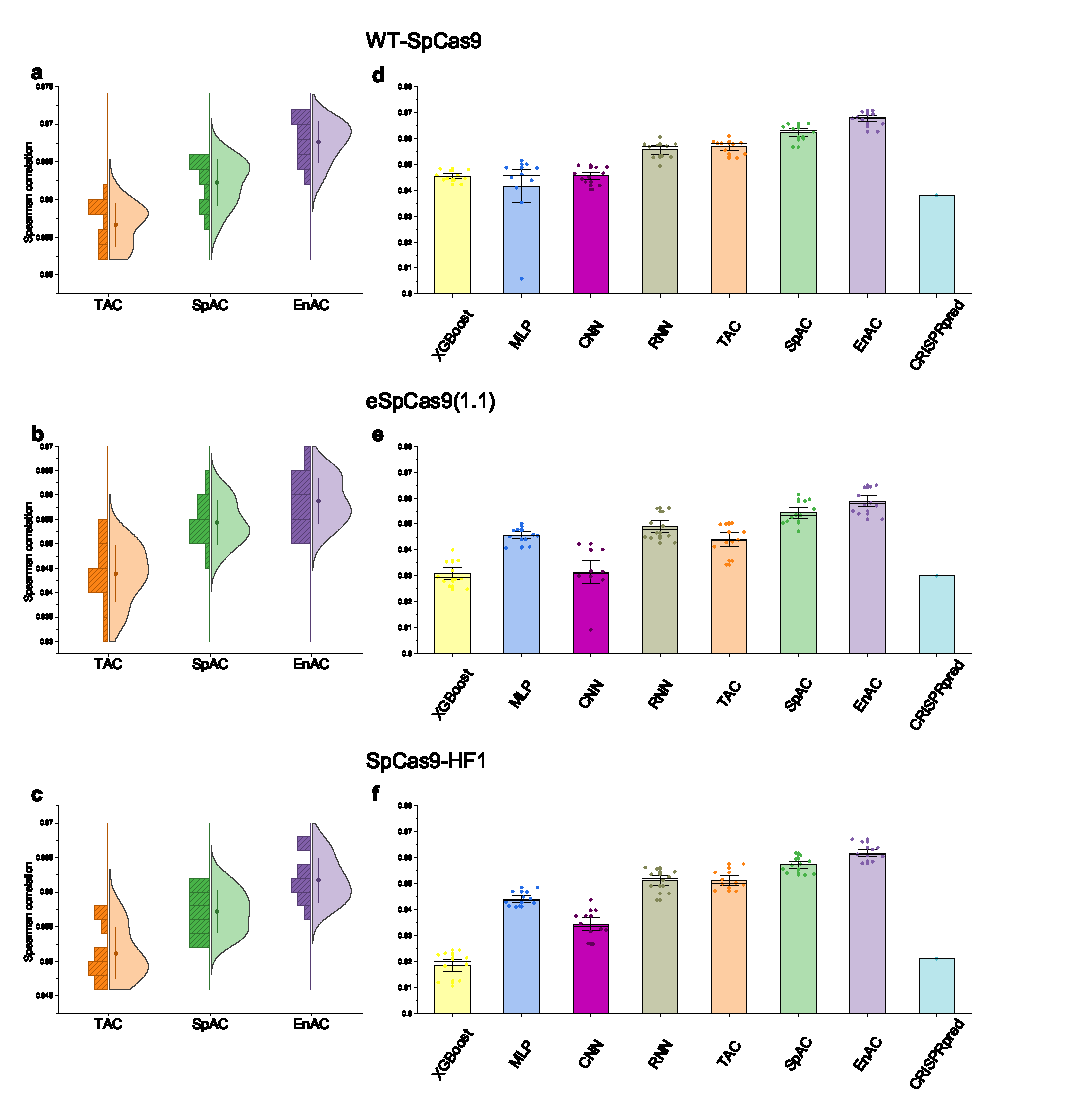
\includegraphics[width=86mm]{baselinewithoutbiofeat.eps}}
    \caption{In the absence of hand-crafted biological features, performance of different algorithms for sgRNA activity prediction. 
    (a)-(c) The performance of Temporal AttCRISPR, Spatial AttCRISPR and Ensemble AttCRISPR. 
    The half-violin plots show the mean and distribution of the Spearman correlation coefficient between predicted and measured sgRNA activity scores over all tests. 
    (d)-(f) In the absence of hand-crafted biological features, the performance of all prediction methods in these datasets as far as we know. 
    The $mean \pm s.d.$ of the Spearman correlation coefficient between predicted and measured sgRNA activity scores are shown in the bar plots.}\label{fig:06}
\end{figure}

\begin{figure}[!tpb]%figure4
    \centerline{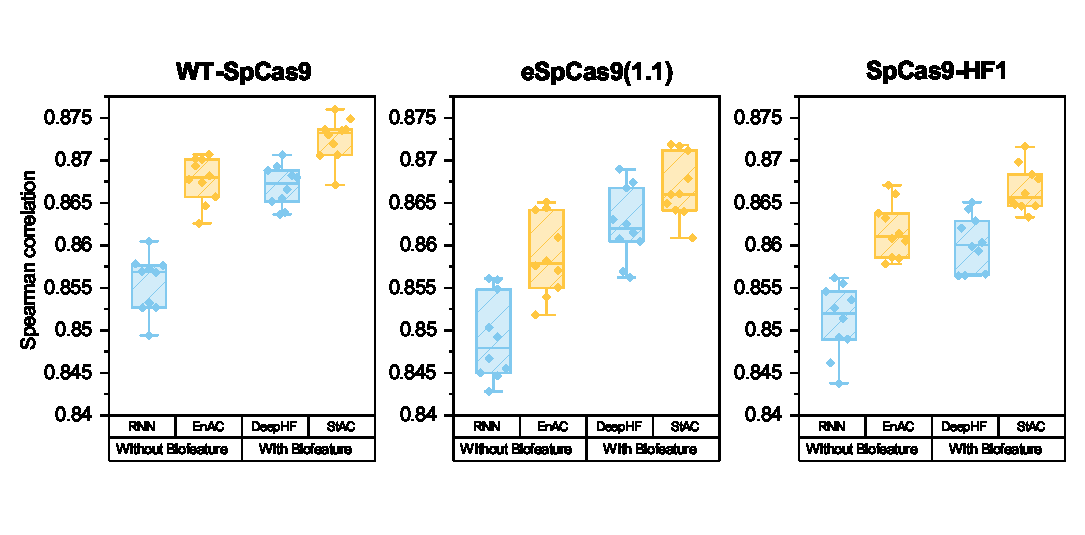
\includegraphics[width=86mm]{baselinewithbiofeat.eps}}
    \caption{
Performance comparisons for the methods before and after integrating with hand-crafted biological features, 
where DeepHF is the RNN integrated with hand-crafted biological features, 
and StAC is the EnAC integrated with hand-crafted biological features. 
The box plot show the mean and distribution of Spearman correlation coefficient between predicted and measured sgRNA activity scores over all tests.
}\label{fig:07}
\end{figure}

We design experiments to address the following questions:
\begin{itemize}
    \item 
    In the absence of hand-crafted biological features, whether the stacking of method in spatial domain and temporal domain can get better performance then use these method alone? 
    $\rightarrow$ Section~\ref{section:stacking}
    \item 
    How does AttCRISPR perform compared to current state-of-the-art methods, covering both conventional machine learning and deep-learning models? 
    $\rightarrow$ Section~\ref{section:comparison}
    \item 
    How can researcher understand the decisions made by AttCRISPR locally and globally, based on attention mechanisms? 
    $\rightarrow$ Section~\ref{section:interpretability}
    \vspace*{1pt}
\end{itemize}

\subsection{Model building and stacking}\label{section:stacking}

In Table~\ref{Tab:withoutbiofeature}, we list the performance of methods in spatial or temporal domain and the stacking of methods. 
Temporal AttCRISPR, TAC for short, achieved Spearman correlation coefficients of 0.857, 0.844, 0.851 respectively in above three dataset. 
Spatial AttCRISPR, SpAC for short, corresponds to 0.862, 0.854, 0.857. In the absence of hand-crafted biological features. 
Ensemble AttCRISPR achieve the best performance of our knowledge, corresponds to 0.868, 0.859, 0.862. 

In addition, in Table~\ref{Tab:withoutbiofeature}, the performance of other methods without using hand-crafted biological features, are also recorded. 
Regardless of the method we developed, RNN reported by \citeauthor{wang2019optimized}, which can be categorized as the method in temporal domain, 
is the most predictive with Spearman correlation coefficients of 0.856, 0.849, 0.851. 
It's obvious that the ensemble AttCRISPR is better at prediction (Figure~\ref{fig:06} (a-c)). 
Furthermore, the prediction ability of models could be boosted by addition of other hand-crafted biological features, which can't be obtained directly by sequence information. 

Further experiment is designed to compare the performance of standard AttCRISPR (hand-crafted biological features are used to improve performance of ensemble AttCRISPR)
 and DeepHF, which is a current state-of-the-art method.
\begin{table}[!tpb]
    \processtable{
    Performance comparisons for different methods in the absence of hand-crafted biological features 
    (take Spearman correlation coefficient as evaluation index)\label{Tab:withoutbiofeature}} 
    {\begin{tabular}{@{}lccc@{}}\toprule
        Method & WT-SpCas9 & eSpCas9(1.1) & SpCas9-HF1\\\midrule
        XGBoost$^*$ & 0.845 & 0.831 & 0.818\\
        MLP$^*$ & 0.842 & 0.846 & 0.844\\
        CNN$^*$ & 0.846 & 0.831 & 0.834\\
        RNN$^*$ & 0.856 & 0.849 & 0.851\\
        TAC & 0.857 & 0.844 & 0.851\\
        SpAC & 0.862 & 0.854 & 0.857\\
        EnAC & \textbf{0.868} & \textbf{0.859} & \textbf{0.862}\\
        CRISPRpred(SEQ)$^{\#}$ & 0.838 & 0.830 & 0.821\\
        \botrule
    \end{tabular}}{}
    \processtable{
    Performance comparisons for the methods before and after integrating with hand-crafted biological features
(take Spearman correlation coefficient as evaluation index)\label{Tab:withbiofeature}} 
    {\begin{tabular}{lcccccc}\toprule
        & \multicolumn{2}{c}{WT-SpCas9} & \multicolumn{2}{c}{eSpCas9(1.1)} & \multicolumn{2}{c}{SpCas9-HF} \\ 
        \cmidrule(lr){2-3} \cmidrule(lr){4-5} \cmidrule(lr){6-7} \noalign{\smallskip} 
        Method & Mean  & \begin{tabular}[c]{@{}l@{}}Std Dev\\ ($\times 10^{-3}$)\end{tabular} & Mean & \begin{tabular}[c]{@{}l@{}}Std Dev\\ ($\times 10^{-3}$)\end{tabular} & Mean & \begin{tabular}[c]{@{}l@{}}Std Dev\\ ($\times 10^{-3}$)\end{tabular} \\ \hline
        RNN$^*$ & 0.856 & 3.33 & 0.849 & 5.00 & 0.851 & 4.11 \\
        EnAC   & 0.868 & 2.66 & 0.859 & 4.66 & 0.862 & 3.19 \\
        DeepHF$^*$ & 0.867 & \textbf{2.37} & 0.862 & 4.24 & 0.860 & 3.21 \\
        StAC   & \textbf{0.872} & 2.55 & \textbf{0.867} & \textbf{3.71} & \textbf{0.867} & \textbf{2.65} \\
     \botrule
\end{tabular}}\footnotesize\setlength{\parindent}{2em}{\emph{Note}: 
The method with superscript of $^*$ and $^{\#}$ is reported by \citeauthor{wang2019optimized} and \citeauthor{MuhammadRafid2020} respectively. 
In the tables, we use the results reported in the relevant papers as the performance of the method directly.}
\end{table}

\subsection{Performance comparison}\label{section:comparison}

\begin{figure*}[!tpb]
    \centerline{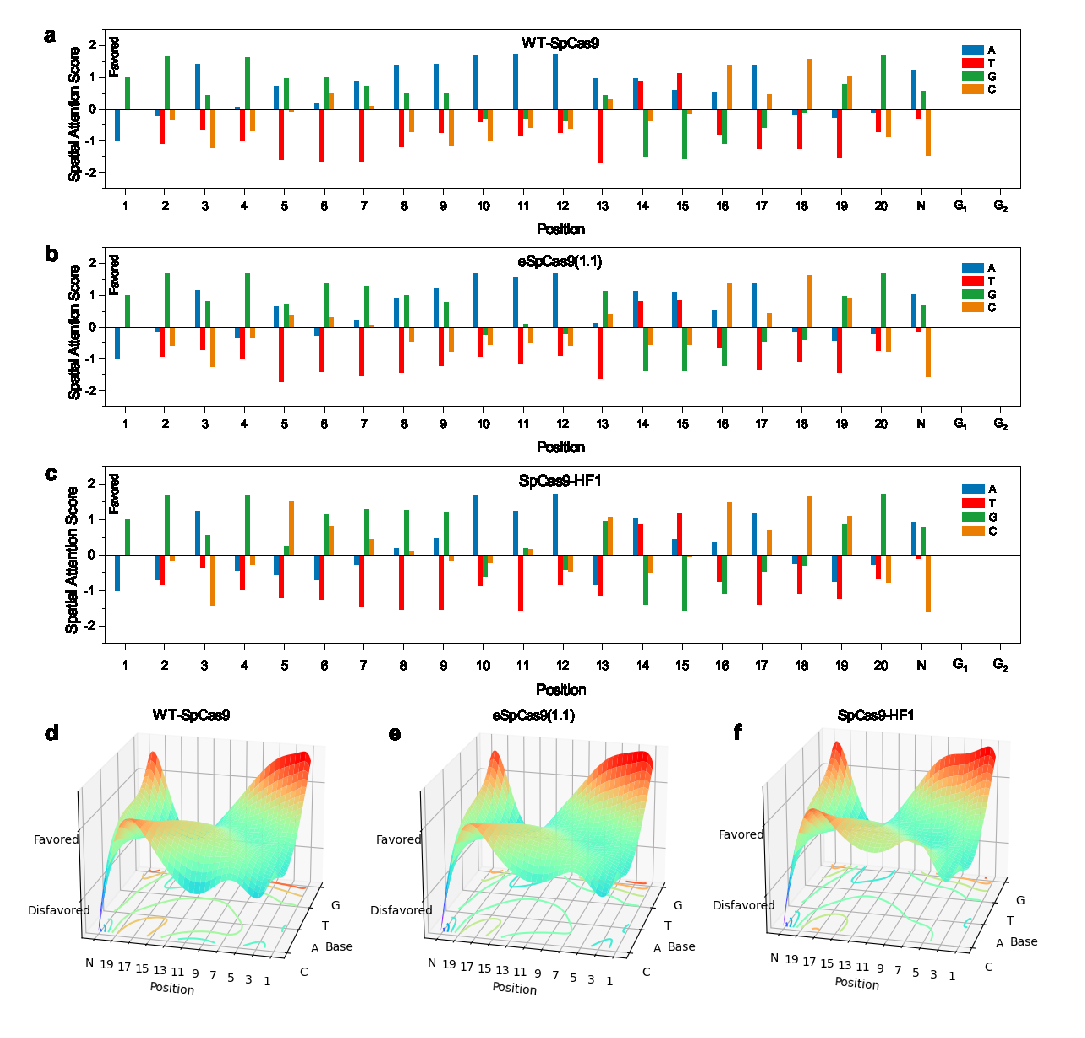
\includegraphics[width=178mm]{spatialattention.eps}}
    \caption{Preference for each position-dependent nucleotide on the sgRNA sequence. 
(a)-(c) Bars show the score of preference after standardization, and the higher the number, the more positive it is for activity of sgRNA. 
The numbers below indicated the position of the nucleotides on-target DNA. 
(d)-(f) Preference surfaces for each position-dependent nucleotide fitted with Bézier surfaces. 
Each position-dependent nucleotide is a control point. 
The coordinates of the control points on the vertical axis represent the degree of preference, 
and the higher the position-dependent nucleotide corresponding to the control point is, the more positive it is for the activity of sgRNA.
The contour plots at the bottom show the area of position-dependent nucleotides which have different contribution to the activity of sgRNA. 
}\label{fig:spatialattention}
\end{figure*}

In order to validate the conclusion that integrating with hand-crafted biological features can improve the predictive performance of methods, 
we follow Equation~(\ref{eq:20}) to modify the ensemble method and design the control experiment using the same strategy. 
What's more, we compare the standard AttCRISPR and DeepHF (Table~\ref{Tab:withbiofeature}).

As shown in Table~\ref{Tab:withbiofeature}, in the absence of hand-crafted biological features, AttCRISPR has significant advantages over DeepHF in predictability. 
Further, integration with the hand-crafted biological features can also improve the performance of AttCRISPR, and achieve Spearman correlation coefficients of 0.872, 0.867 and 0.867 for WT-SpCas9, eSpCas9(1.1) and SpCas9-HF1, respectively. Meanwhile, DeepHF achieve 0.867, 0.862 and 0.860, respectively. 
After integrating with biological features, the performance gap between AttCRISPR and DeepHF is shortened, while AttCRISPR still has better performance. In addition, we also compare the standard deviation of data obtained in ten tests, which are also shown in Table~\ref{Tab:withbiofeature}. 
It reveal that AttCRISPR is more stable than DeepHF.

\subsection{Interpretability of the AttCRISPR}\label{section:interpretability}

In the following sections, we will analyze the insight into activity of sgRNA bring through the attention mechanism at both global and local levels 
to validate the attention module in the AttCRISPR can help us to understand the decisions. 
\subsubsection{Global interpretability}

At global level, an important question we expect AttCRISPR to answer is which nucleotide it prefers at each position on the sequence. 
In fact, \citeauthor{wang2019optimized} has already answered this question in detail with the DeepSHAP method.
Leaving aside nucleotides, just consider the importance of each position, the method of \citeauthor{Liu2019} have gone some way too. 
While our method is not based on the post hoc explanations techniques and input perturbations, the only work we need to do is to get the first-order preference $A$ generated by the attention module.
Specifically, we use the first-order preference $A_s$ generated by the spatial attention module instead of  $\tilde{A}$ generated by the temporal attention module. 
The latter is in a higher dimensional dense space which make it difficult to understand. 
In practice, we input every sgRNA into the spatial AttCRISPR, in order to obtain the $A_s$ from the spatial attention module and take its mean value. 
Then we rescale it through Z-score to obtain a standardization value and the final result is shown in Figure~\ref{fig:spatialattention}. 

As shown in Figure~\ref{fig:spatialattention}, we captured the preference for each position-dependent nucleotide on the sgRNA sequence. 
The result revealed that A and G typically have a positive contribution to the activity of sgRNA, while T typically have a negative contribution. 
It is agree with previous conlusion that when Cas9 is binding sgRNA, it prefer the one containing purines to pyrimidines \citep{wang2014genetic}. 
In addition, global interpretability also pointed out that distinct from other nucleotides, G is strongly favored at position 20. 
This is consistent with the conclusions of several other reports \citep{Wong2015,Doench2014}.

Furthermore, the preference of the nucleotide at the same position doesn't change dramatically with the Cas9 nucleases, 
while we still notice that compared with the other two datasets, 
C makes a more positive contribution to the activity of sgRNA with the SpCas9-HF1 especially in the position 5, which is evident in Figure~\ref{fig:spatialattention} (d-f). 

The above discussion shows that, in the task of sgRNA activity prediction, 
attention mechanism can help us understand the decision made by AttCRISPR and reveal the insight into activity of sgRNA. 

\subsubsection{Local interpretability}\label{section:local}

At local level, we analyze a case (consisting of three sgRNAs as Table~\ref{Tab:optimum} show), 
then we expect AttCRISPR to answer two imortant questions based on the local interpretability. 
First, how can we optimize a sgRNA to have more on-target activity. 
Second, what are the reasons for the low activity of the sgRNA. 

For the first question, we input the least-active sgRNA in Table~\ref{Tab:optimum} (with the index of 8493 and the activity of 0.831, call source sgRNA for convenience) into the temporal AttCRISPR. 
The score of each position is obtained based on Equation~(\ref{eq:05}) (the calculated symbol with $W$ is Hadamard product instead of dot product, in order to achieve the result in vector form), 
and the results are shown in Figure~\ref{fig:opt}. 
Acording to Figure~\ref{fig:opt}, scores at position 14 and 16 of source sgRNA are significantly below the base line 
(in fact, the scores at position 6 and 11 is also noteworthy, however, we don't find sgRNA in the dataset for comparison). 
If replaced the T at position 14 with C, would generate the same sgRNA as the one with index of 8491, which is with a activity value of 0.861. 
If replaced the T at position 16 with C, would generate the same sgRNA as the one with index of 8492, which is with a activity value of 0.869. 
Therefore, we could conclude that the local interpretability is helpful for us to optimize the sgRNA without exhaustively search.

The second question we expect AttCRISPR to answer is why it give two low scores at position 14 and 16. 
In practice, we will try to answer this question with second-order preference. 
Let AttCRISPR output the second-order preference matrix $B$ corresponding to the source sgRNA, and show it in Figure~\ref{fig:heatmap}. 
It is obvious that a few unusual bright spots appear in the red box in Figure~\ref{fig:heatmap}, 
which show that the nucleotide at position 15 has a great effect on the score of position 14 and 16 (instead of position 13 or 17, which corresponding position are relatively dim in color). 
As shown in Table~\ref{Tab:optimum}, in source sgRNA there are three consecutive Ts at position 14, 15 and 16, and this may reveal that multiple consecutive Us on sgRNA would leads to low on-target activity of sgRNA, which is consistent with earlier report \citep{wu2014genome-wide}. 

\section{Discussion}

In this article, we have developed a new prediction method, called AttCRISPR for the activity of sgRNA. 
We take the ensemble of both spatial and temporal domain to predict the on-target activity of sgRNA. 
Throught ablation analysis and testing a series of possible network structure, we demonstrate that the ensemble method performs better than other methods on this task. 
In addition, we apply attention modules in both the spatial and temporal parts of AttCRISPR, 
and design two experiments combined with some early reports to prove that attention mechanisms can help researcher understand the decisions made by model which make it easy to optimize low activity sgRNA without exhaustively search. 

In Section~\ref{section:stacking}, we have tested both spatial and temporal domain AttCRISPR, and CNN (method in spatial domain), RNN (method in temporal domain) which reported by \citeauthor{wang2019optimized} in the absence of hand-crafted biological features. 
A worth noticing point is that there is a gap between spatial AttCRISPR and CNN, though the performance of temporal AttCRISPR is basically the same as that of RNN. 
We suspect there are two possible reasons. 
One is that attention modules can significantly improve the performance of the model, which is short of experimental validation, 
and the other is that the performance of the method in spatial domain is underestimated. 

In Section~\ref{section:comparison}, also integrating with hand-srafted biological features to improve the predictive performance, the performance gap between AttCRISPR and DeepHF is shortened, while AttCRISPR still has better performance. 
This may be a natural belief that with the primary biological sequence we can predict the functional and structural information. 
Therefore, there is a limit to the performance improvement by integrating with hand-srafed biological features. 

As shown in Figure~\ref{fig:heatmap}, we note that the brightness at coordinates (14, 15) and (16, 15) exceeds (14, 13) and (16, 17). 
In other words, there are two unusual bright spots at coordinates (14, 15) and (16, 15). 
This could explain that the nucleotide trimer at position 14, 15, 16 has a great influence on the decision made by AttCRISPR. 
We believe that we can use a carefully designed $3\times 3$ convolution kernel, and move it along the diagonal of the second-order preference matrix $B$, 
in order to find all kind of nucleotide trimer that have a great influence on the decision made by AttCRISPR. 
Further experiments may be need to validate. 

Current architecture of AttCRISPR focuses on predicting the on-target activity of conventional sgRNA which have a PAM based on NGG. 
However it can be extended to other Cas9 species, variants or off-target task easily. 

\section{Conclusion}

\begin{table}[!tpb]
    \processtable{Three sgRNA and their activity \label{Tab:optimum}} 
    {\begin{tabular}{@{}lll@{}}\toprule
        Index & sgRNA & Activity \\\midrule
        8493 & ACATGACTTTGGATTTCCCCAGG & 0.831\\
        8492 & ACATGACTTTGGATTCCCCCAGG & 0.869\\
        8491 & ACATGACTTTGGACTTCCCCAGG & 0.861\\
        \botrule
    \end{tabular}}\footnotesize\setlength{\parindent}{2em}{\emph{Note}: 
    \emph{Activity} of sgRNA represents the activity reported in WT-SpCas9 dataset (Supplementary Data 1). }
\end{table}
\begin{figure}[!tpb]
    \centerline{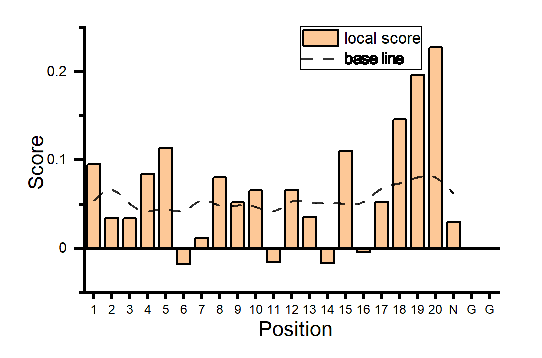
\includegraphics[width=86mm]{local0.eps}}
    \caption{
The scores of sgRNA with index of 8493 obtained by the temporal AttCRISPR. 
The bar plot reveals the score at each position at local level, while the line of dashes reveals the scores at global level. 
At global level we calculated the scores of all sgRNA, then average the scores at each position to obtain the global level which can be used as base line and is helpful to judge the relative height of the scores. 
}\label{fig:opt}
\end{figure}

\begin{figure}[!tpb]
    \centerline{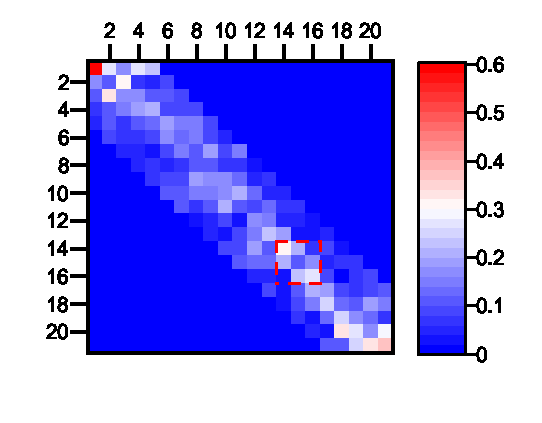
\includegraphics[width=86mm]{secondorder.eps}}
    \caption{The visualization of second-order preference matrix $B$, 
the elements in the $i$-th row and the $j$-th column represent the influence of nucleotide at position $j$ when generate the first-order preference $\tilde{A}$ at position $i$. 
The warmer the color, the more important it is. 
In the red box, a few unusual bright spots appear. 
To be more specific, the nucleotide at position 15 has a great effect on the first-order preference at positon 14 and 16.
}\label{fig:heatmap}
\end{figure}
In this paper, we develop AttCRISPR, an ensemble method of both spatial method and temporal method follow the stacking strategy with strong interpretability. 
AttCRISPR prove that the ensemble methods have a better performance in the datasets of DeepHF
and can compete with current state-of-the-art methods. 
In addition, AttCRISPR apply attention mechanisms in both the temporal and spatial part, 
and we explain the decisions made by AttCRISPR through the attention module which is consistent with earlier reports. 
Further, we also discovered that the output of the attention module can be used to optimize the low-activity sgRNA without exhaustively search, 
and our optimization results are verified with available experimental data. 
To our knowledge, this is the first time that the attentional mechanim is used to reveal the reasons influencing on-target activity of sgRNA, and assist sgRNA design.  


\section*{Funding}

This work was partially supported by grants from the National Key R\&D Program of China (2019YFA0110802 and 2019YFA0802800).
\\\\\emph{Conflict of Interest}: none declared.\vspace*{-12pt}

\bibliographystyle{natbib}
\bibliography{document}

\end{document}